\documentclass[10pt,a4paper,spanish]{beamer}

\usepackage[spanish]{babel}
\usepackage[utf8]{inputenc}
\usepackage{amsmath, amsthm}
\usepackage{amsfonts, amssymb, latexsym}
\usepackage{enumerate}
\usepackage[official]{eurosym}
\usepackage{graphicx}
\usepackage[usenames, dvipsnames]{color}
\usepackage{colortbl}
\usepackage{multirow}
\usepackage{fancyhdr}
\usepackage[all]{xy}
\usepackage{minted}
\usepackage{tikz}
\usepackage{pgfplots}
\usepackage{algpseudocode}
\usepackage{listings}
\usepackage[math]{iwona}
\usepackage[T1]{fontenc}
\usepackage{inconsolata}



\usepackage[pdftex, bookmarks=true,
	bookmarksnumbered=false, % true means bookmarks in
	% left window are numbered
	bookmarksopen=false,     % true means only level 1
	% are displayed.
	colorlinks=true,
linkcolor=webblue]{hyperref}

\definecolor{webgreen}{rgb}{0, 0.5, 0} % less intense green
\definecolor{webblue}{rgb}{0, 0, 0.5}  % less intense blue
\definecolor{webred}{rgb}{0.5, 0, 0}   % less intense red
\definecolor{dblackcolor}{rgb}{0.0,0.0,0.0}
\definecolor{dbluecolor}{rgb}{.01,.02,0.7}
\definecolor{dredcolor}{rgb}{0.8,0,0}
\definecolor{dgraycolor}{rgb}{0.30,0.3,0.30}


%%%%% Para cambiar el tipo de letra en el título de la sección %%%%%%%%%%%
\chapterfont{\fontfamily{pag}\selectfont} %% for chapter if you want
\sectionfont{\fontfamily{pag}\selectfont}
\subsectionfont{\fontfamily{pag}\selectfont}
\subsubsectionfont{\fontfamily{pag}\selectfont}

\renewcommand{\labelenumi}{\arabic{enumi}. }
\renewcommand{\labelenumii}{\labelenumi\alph{enumii}) }
\renewcommand{\labelenumiii}{\labelenumii\roman{enumiii}: }

\newmintedfile[myCpp]{cpp}{
	linenos,
	numbersep=5pt,
	gobble=0,
	frame=lines,
	framesep=2mm,
	fontsize=\footnotesize
}

\newmintedfile[myLex]{bash}{
	linenos,
	numbersep=5pt,
	gobble=0,
	frame=lines,
	framesep=2mm,
	breaklines=true,
	fontsize=\footnotesize
}

\newmintedfile[myLatex]{tex}{
	linenos,
	numbersep=5pt,
	gobble=0,
	frame=lines,
	framesep=2mm,
	tabsize=3,
}

\newmintedfile[myHtml]{html}{
	linenos,
	numbersep=5pt,
	gobble=0,
	frame=lines,
	framesep=2mm,
	tabsize=3,
}

% Tema para la presentación
\mode<presentation>{\usetheme{Madrid}}
\title{ZigBee}
\author{David Sánchez Jiménez}

\begin{document}
\frame{\titlepage}

% Primera transparencia
\begin{frame}
	\frametitle{Definición}
	\begin{columns}
		\begin{column}{6cm}
			ZigBee es un estándar de comunicaciones inalámbricas diseñado por la ZigBee Alliance compuesto por un conjunto de protocolos de alto nivel de comunicación inalámbrica para su utilización con radiodifusión digital de bajo consumo. \\

			\vspace{0.5cm}
			Esta basado en el estándar IEEE 802.15.4 de redes WPAN y tiene como objetivo aplicaciones que requieren comunicaciones seguras con baja tasa de envío de datos y maximización de la vida util de las baterías.
		\end{column}
		\begin{column}{5cm}
			\begin{center}
				\includegraphics[height=3.5cm]{imagenes/1.png}
			\end{center}
		\end{column}
	\end{columns}
\end{frame}

% Segunda Transparencia
\begin{frame}
	\frametitle{Pila de protocolos ZigBee}
	\begin{columns}
		\begin{column}{6cm}
			Las dos primeras capas de la pila de protocolos se basan en el nivel físico y MAC definidos en el estandar IEEE 802.15.4-2003.\\

			\vspace{0.5cm}
			Las capas superiores están definidas por la ZigBee Alliance y se corresponden a las capas de red y de aplicación las cuales contienen los perfiles de uso, ajustes de seguridad y mensajería.
		\end{column}
		\begin{column}{6cm}
			\begin{center}
				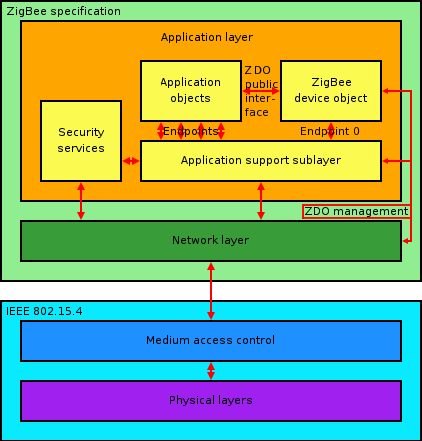
\includegraphics[height=6cm]{imagenes/2.png}
			\end{center}
		\end{column}
	\end{columns}
\end{frame}

% Tercera Transparencia
\begin{frame}
	\frametitle{Pila de protocolos ZigBee}
	\begin{columns}
		\begin{column}{6cm}
			Los principales cometidos de la capa de red son:
			\begin{itemize}
				\item Permitir el correcto uso del subnivel MAC.
				\item Ofrecer un interfaz adecuado para su uso por parte del nivel inmediatamente superior
			\end{itemize}

			\vspace{0.5cm}
			Por su parte la Capa de Aplicación se encarga de los procedimientos de control, seguridad y de los objetos de aplicación.
		\end{column}
		\begin{column}{6cm}
			\begin{center}
				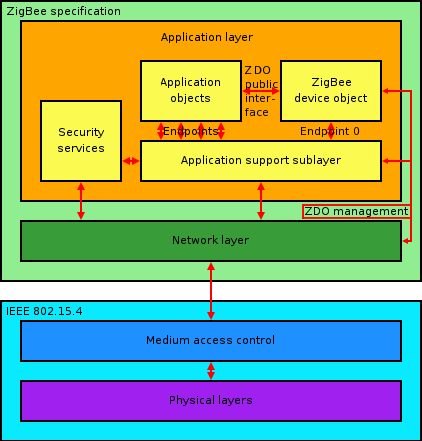
\includegraphics[height=6cm]{imagenes/2.png}
			\end{center}
		\end{column}
	\end{columns}
\end{frame}

% Cuarta Transparencia
\begin{frame}
	\frametitle{Topologías de red}
	ZigBee permite tres topologías de red:
	\begin{block}{}
		\begin{itemize}
			\item Topología en estrella: El nodo coordinador se situa en el centro.
			\item Topología en arbol: El nodo coordinador se situa en la raiz.
			\item Topología de malla: Al menos un nodo tendrá más de dos conexiones.
		\end{itemize}
	\end{block}

	\vspace{0.5cm}
	La más usada es la topología de malla debido a que permite que si uno de los nodos falla y se cae, el coordinador rehace todos los caminos y la comunicación entre los demás nodos puede continuar sin ningun problema.
\end{frame}

% Han sido diseñadas para conservar la potencia en los nodos ''esclavos'' manteniendolos durante mucho tiempo ''dormido''. Un nodo esclavo se ''despierta'' por una fracción de segundo para confirmar que está ''vivo'' en la red de la que forma parte.

% \begin{frame}
% 	\frametitle{Tipos de Tráfico de Datos}
% 	Los dispositivos ZigBee dirigen tres tipos de tráfico tipicos:
% 	\begin{block}{}
% 		\begin{itemize}
% 			\item Cuando el dato es periódico: La aplicación dicta la proporción, el sensor se activa, chequea los datos y luego desactiva.
% 			\item Cuando el dato es intermitente: La aplicación determina la proporción y el dispositivo necesita sólo conectarse a la red cuando la comunicación se hace necesaria. Este tipo habilita el ahorro óptimo en la energía.
% 			\item Cuando el dato es repetitivo: La proporción es a priori fija. Dependiendo de las hendeduras de tiempo repartidas, los dispositivos operan para las duraciones fijas.
% 		\end{itemize}
% 	\end{block}
% \end{frame}

\begin{frame}
	\frametitle{Tipos de dispositivos}
	Hay tres tipos de dispositivos ZigBee segun su papel en la red:

	\begin{block}{}
		\begin{itemize}
			\item •Coordinador de red: hay uno solo en cada red. Es el que mantiene en todo momento el control del sistema, requiere memoria y capacidad de computación.
			\item • Dispositivo de función completa (FFD): es un router intermediario que transmite datos desde otros dispositivos. Puede operar en todas las topologías y también puede actuar como un cooordinador.
			\item •Dispositivo de función reducida (RFD): Estos son los sensores o actuadores de la red de capacidad y funcionalidad limitada.
		\end{itemize}
	\end{block}
\end{frame}

\begin{frame}
	\frametitle{Aplicaciones}
	Los protocolos ZigBee están definidos para su uso en aplicaciones embebidas con requerimientos muy bajos de transmisión de datos y consumo energético. Se pretende su uso en aplicaciones de propósito general con características auto organizativas y bajo coste ya que la red en su conjunto utilizará una cantidad muy pequeña de energía de forma que cada dispositivo pueda tener una autonomía de hasta 5 años.\\

	\vspace{0.25cm}
	Puede utilizarse para realizar control industrial, albergar sensores empotrados, sensores remotos, recolectar datos, ejercer labores de detección de humo o intrusos, utilizarlos para la automatización o incluso para domótica.
\end{frame}

\begin{frame}
	\frametitle{Ventajas e inconvenientes}
	\begin{block}{Ventajas}
		\begin{itemize}
			\item Ideal para conexiones punto a punto y punto a multipunto.
			\item Óptimo para redes de baja tasa de transferencia de datos.
			\item Cifrado 128-bit AES.
			\item Proporciona larga duración de la batería.
			\item Permite hasta 65.000 nodos en una red.
			\item Son baratos de fabricar.
		\end{itemize}
	\end{block}
	\begin{block}{Inconvenientes}
		\begin{itemize}
			\item La tasa de transferencia es muy baja.
			\item No es compatible con bluetooth.
			\item Tiene menor cobertura porque pertenece a redes inalámbricas de tipo WPAN.
		\end{itemize}
	\end{block}
\end{frame}
\end{document}
